\documentclass[tikz]{standalone}
\usepackage{pgfplots}
\usepackage{xcolor}
\definecolor{brown}{HTML}{8a4e3d}
\definecolor{blue}{HTML}{6d9eeb}
\definecolor{gray}{HTML}{888888}
\definecolor{gold}{HTML}{ffd966}
\pgfplotsset{compat=1.18}

\begin{document}
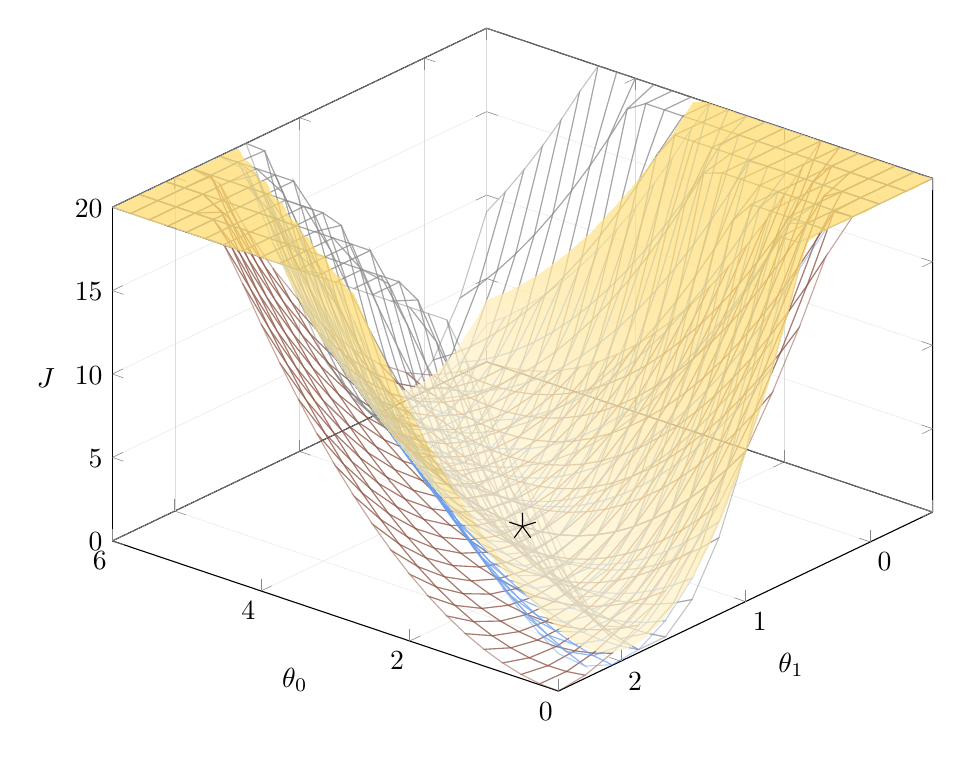
\begin{tikzpicture}
  \begin{axis}[
    view={220}{35},
    xlabel={\(\theta_0\)},
    ylabel={\(\theta_1\)},
    zlabel={\(J\)},
    zlabel style={rotate=-90},
    xmin=0, xmax=6,
    ymin=-0.5, ymax=2.5,
    zmin=0, zmax=20,
    width=12cm,
    height=10cm,
    grid=major,
    major grid style={line width=0.1pt, draw=gray!30},
  ]
    % J₁ as wireframe (parabolic cylinder, valley along θ₀+2θ₁=5)
    \addplot3[
      mesh, color=brown, opacity=0.5,
      domain=0:6, domain y=-0.5:2.5,
      samples=25, samples y=15,
    ] {min((x+2*y-5)^2, 20)};

    % J₂ as wireframe
    \addplot3[
      mesh, color=blue, opacity=0.5,
      domain=0:6, domain y=-0.5:2.5,
      samples=25, samples y=15,
    ] {min((x+3*y-6)^2, 20)};

    % J₃ as wireframe
    \addplot3[
      mesh, color=gray, opacity=0.5,
      domain=0:6, domain y=-0.5:2.5,
      samples=25, samples y=15,
    ] {min((x+4*y-7)^2, 20)};

    % Combined J as solid surface
    \addplot3[
      surf, shader=interp, opacity=0.7,
      colormap={goldmap}{color=(gold!30) color=(gold!80) color=(gold)},
      domain=0:6, domain y=-0.5:2.5,
      samples=40,
    ] {min(((x+2*y-5)^2 + (x+3*y-6)^2 + (x+4*y-7)^2)/3, 20)};

    % Mark minimum at (3, 1, 0)
    \addplot3[only marks, mark=star, mark options={scale=2.5, fill=red}]
      coordinates {(3,1,0)};
  \end{axis}
\end{tikzpicture}
\end{document}
